\section{Bibliografía, datasheets e instrumentos}
\subsection{Bibliografía}
\begin{itemize}[nosep]
    \item Floyd, Thomas L. Principles of Electric Circuits: Conventional Current Version.
    \item Clases teóricas de la asignatura ''Dispositivos Electrónicos''.
    \item Datasheets de los instrumentos proporcionados por los fabricantes.
\end{itemize}
\subsection{Instrumentos}
\begin{center}
\begin{figure}[h!]
  \centering
  \begin{subfigure}[b]{0.4\linewidth}
    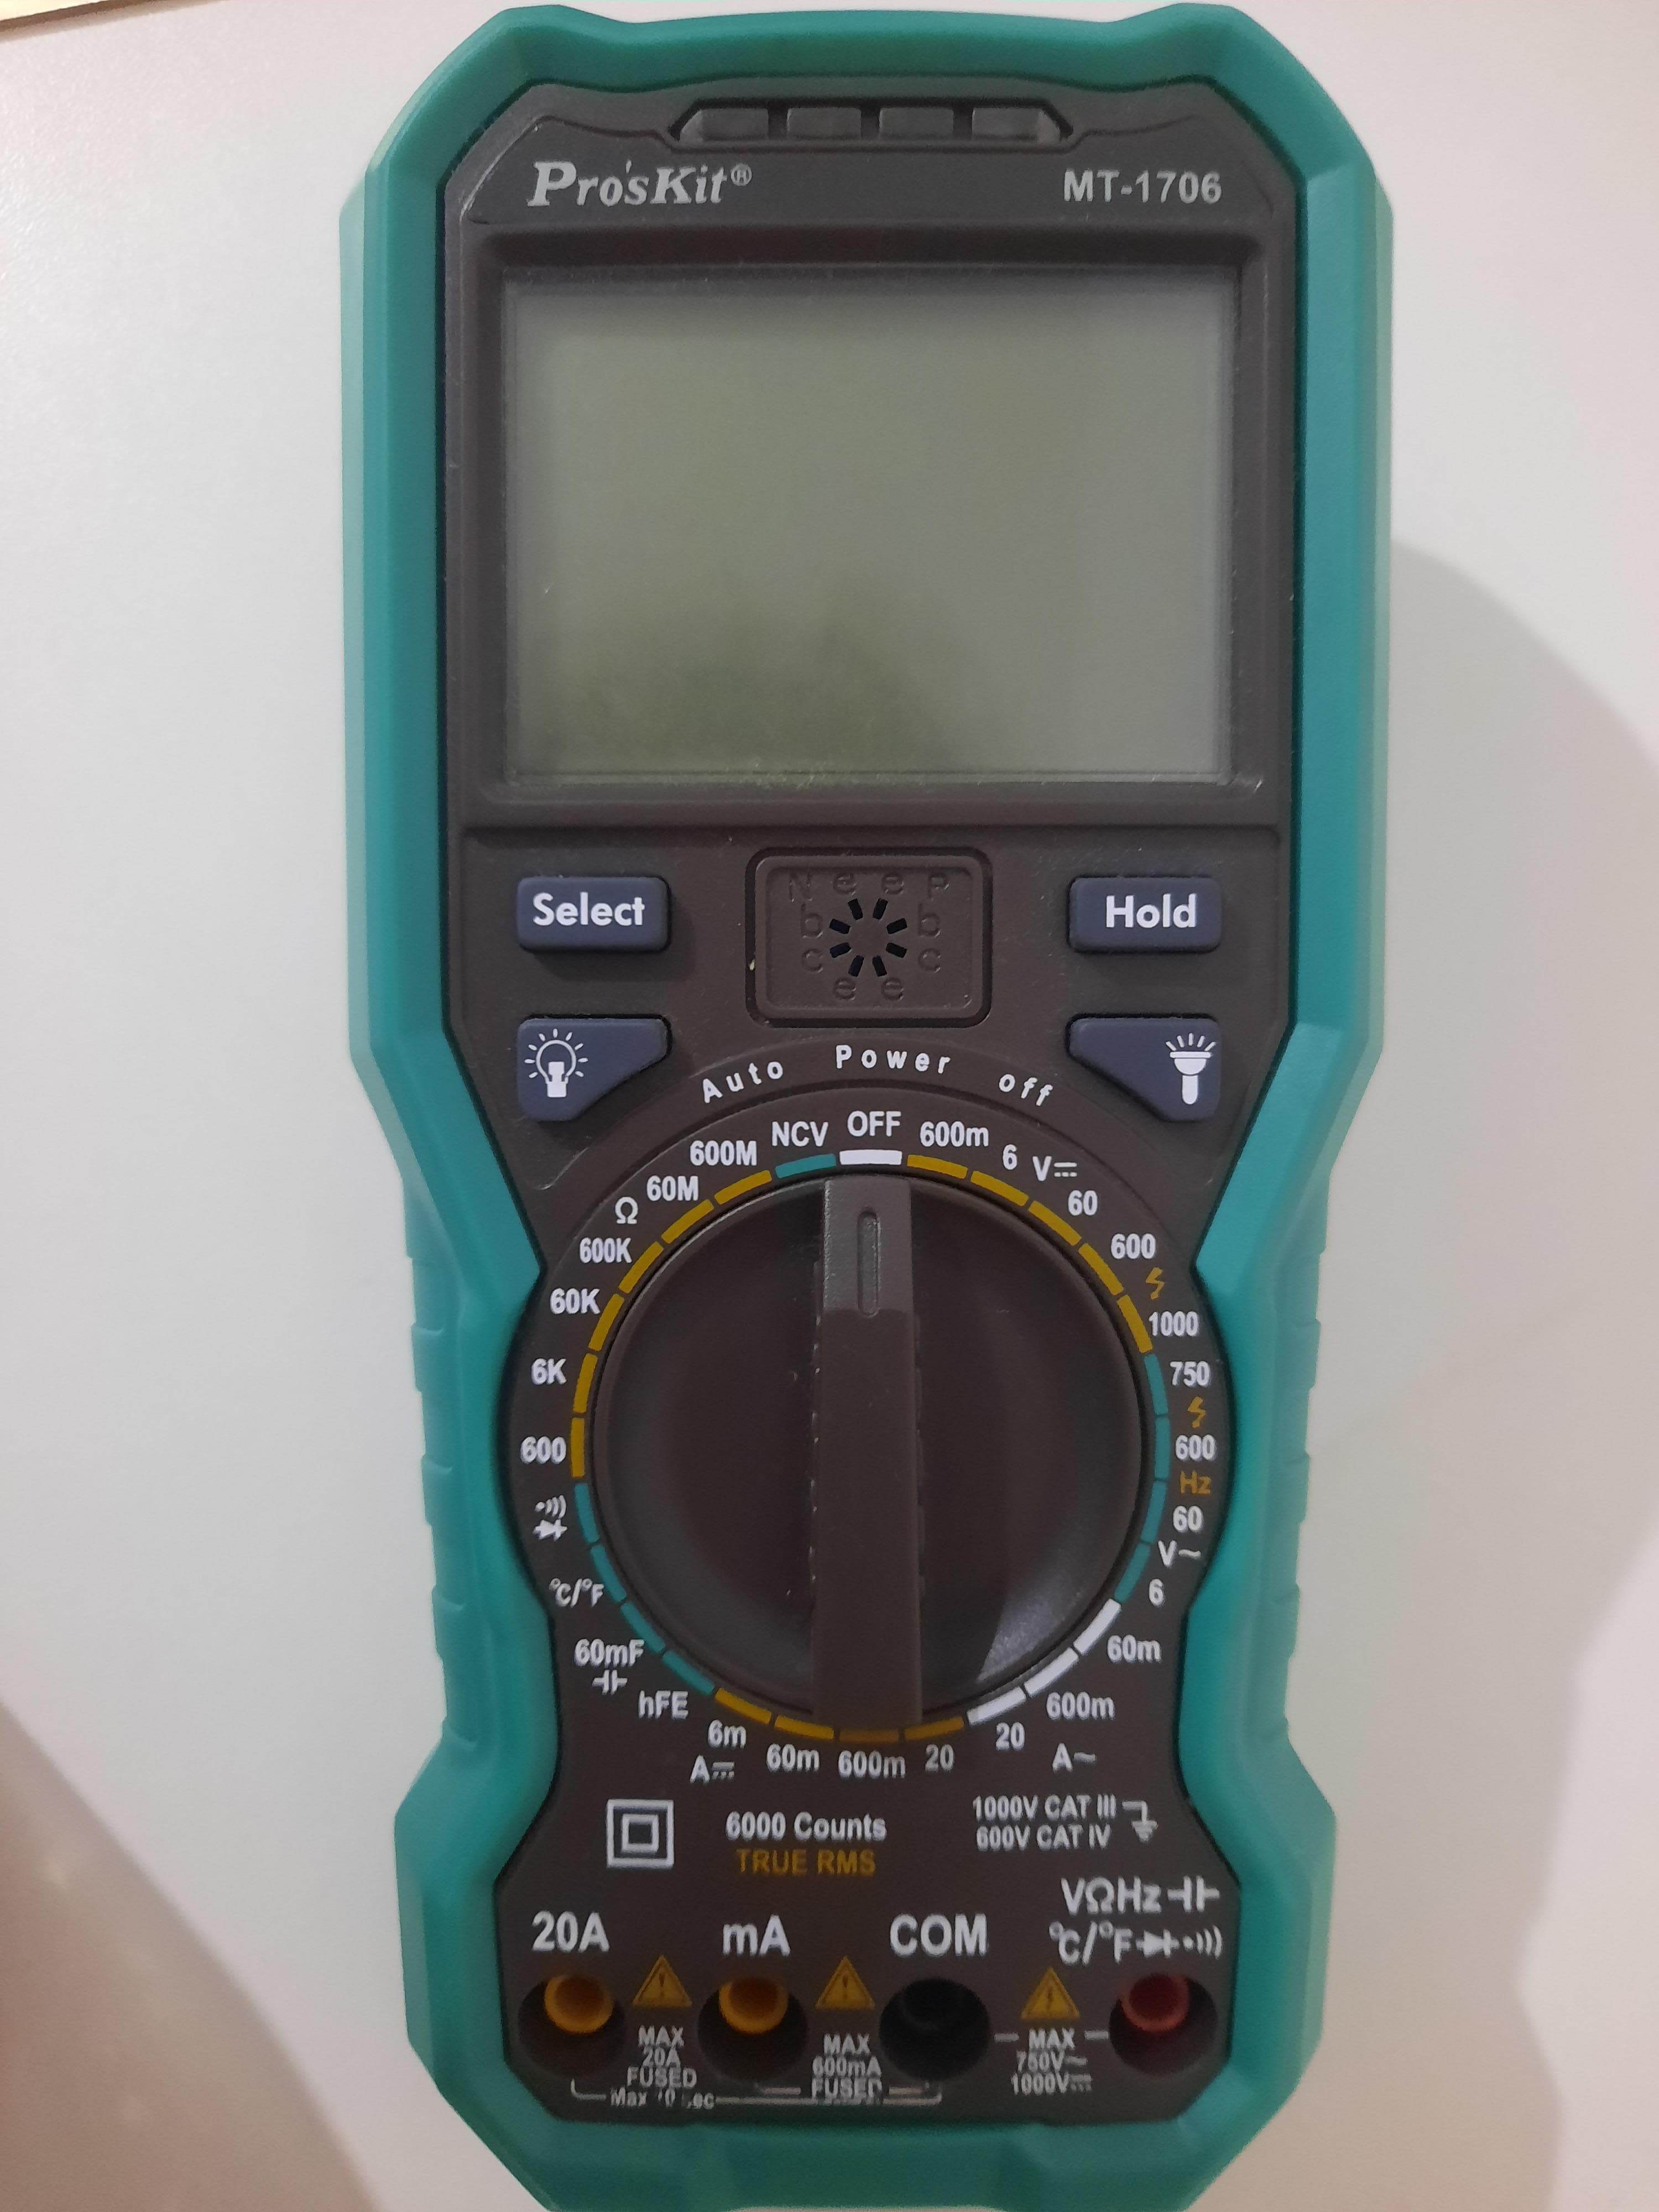
\includegraphics[width=\linewidth]{./imagenes/multimetro.jpg}
    \caption{Multimetro 1}
  \end{subfigure}
  \begin{subfigure}[b]{0.4\linewidth}
    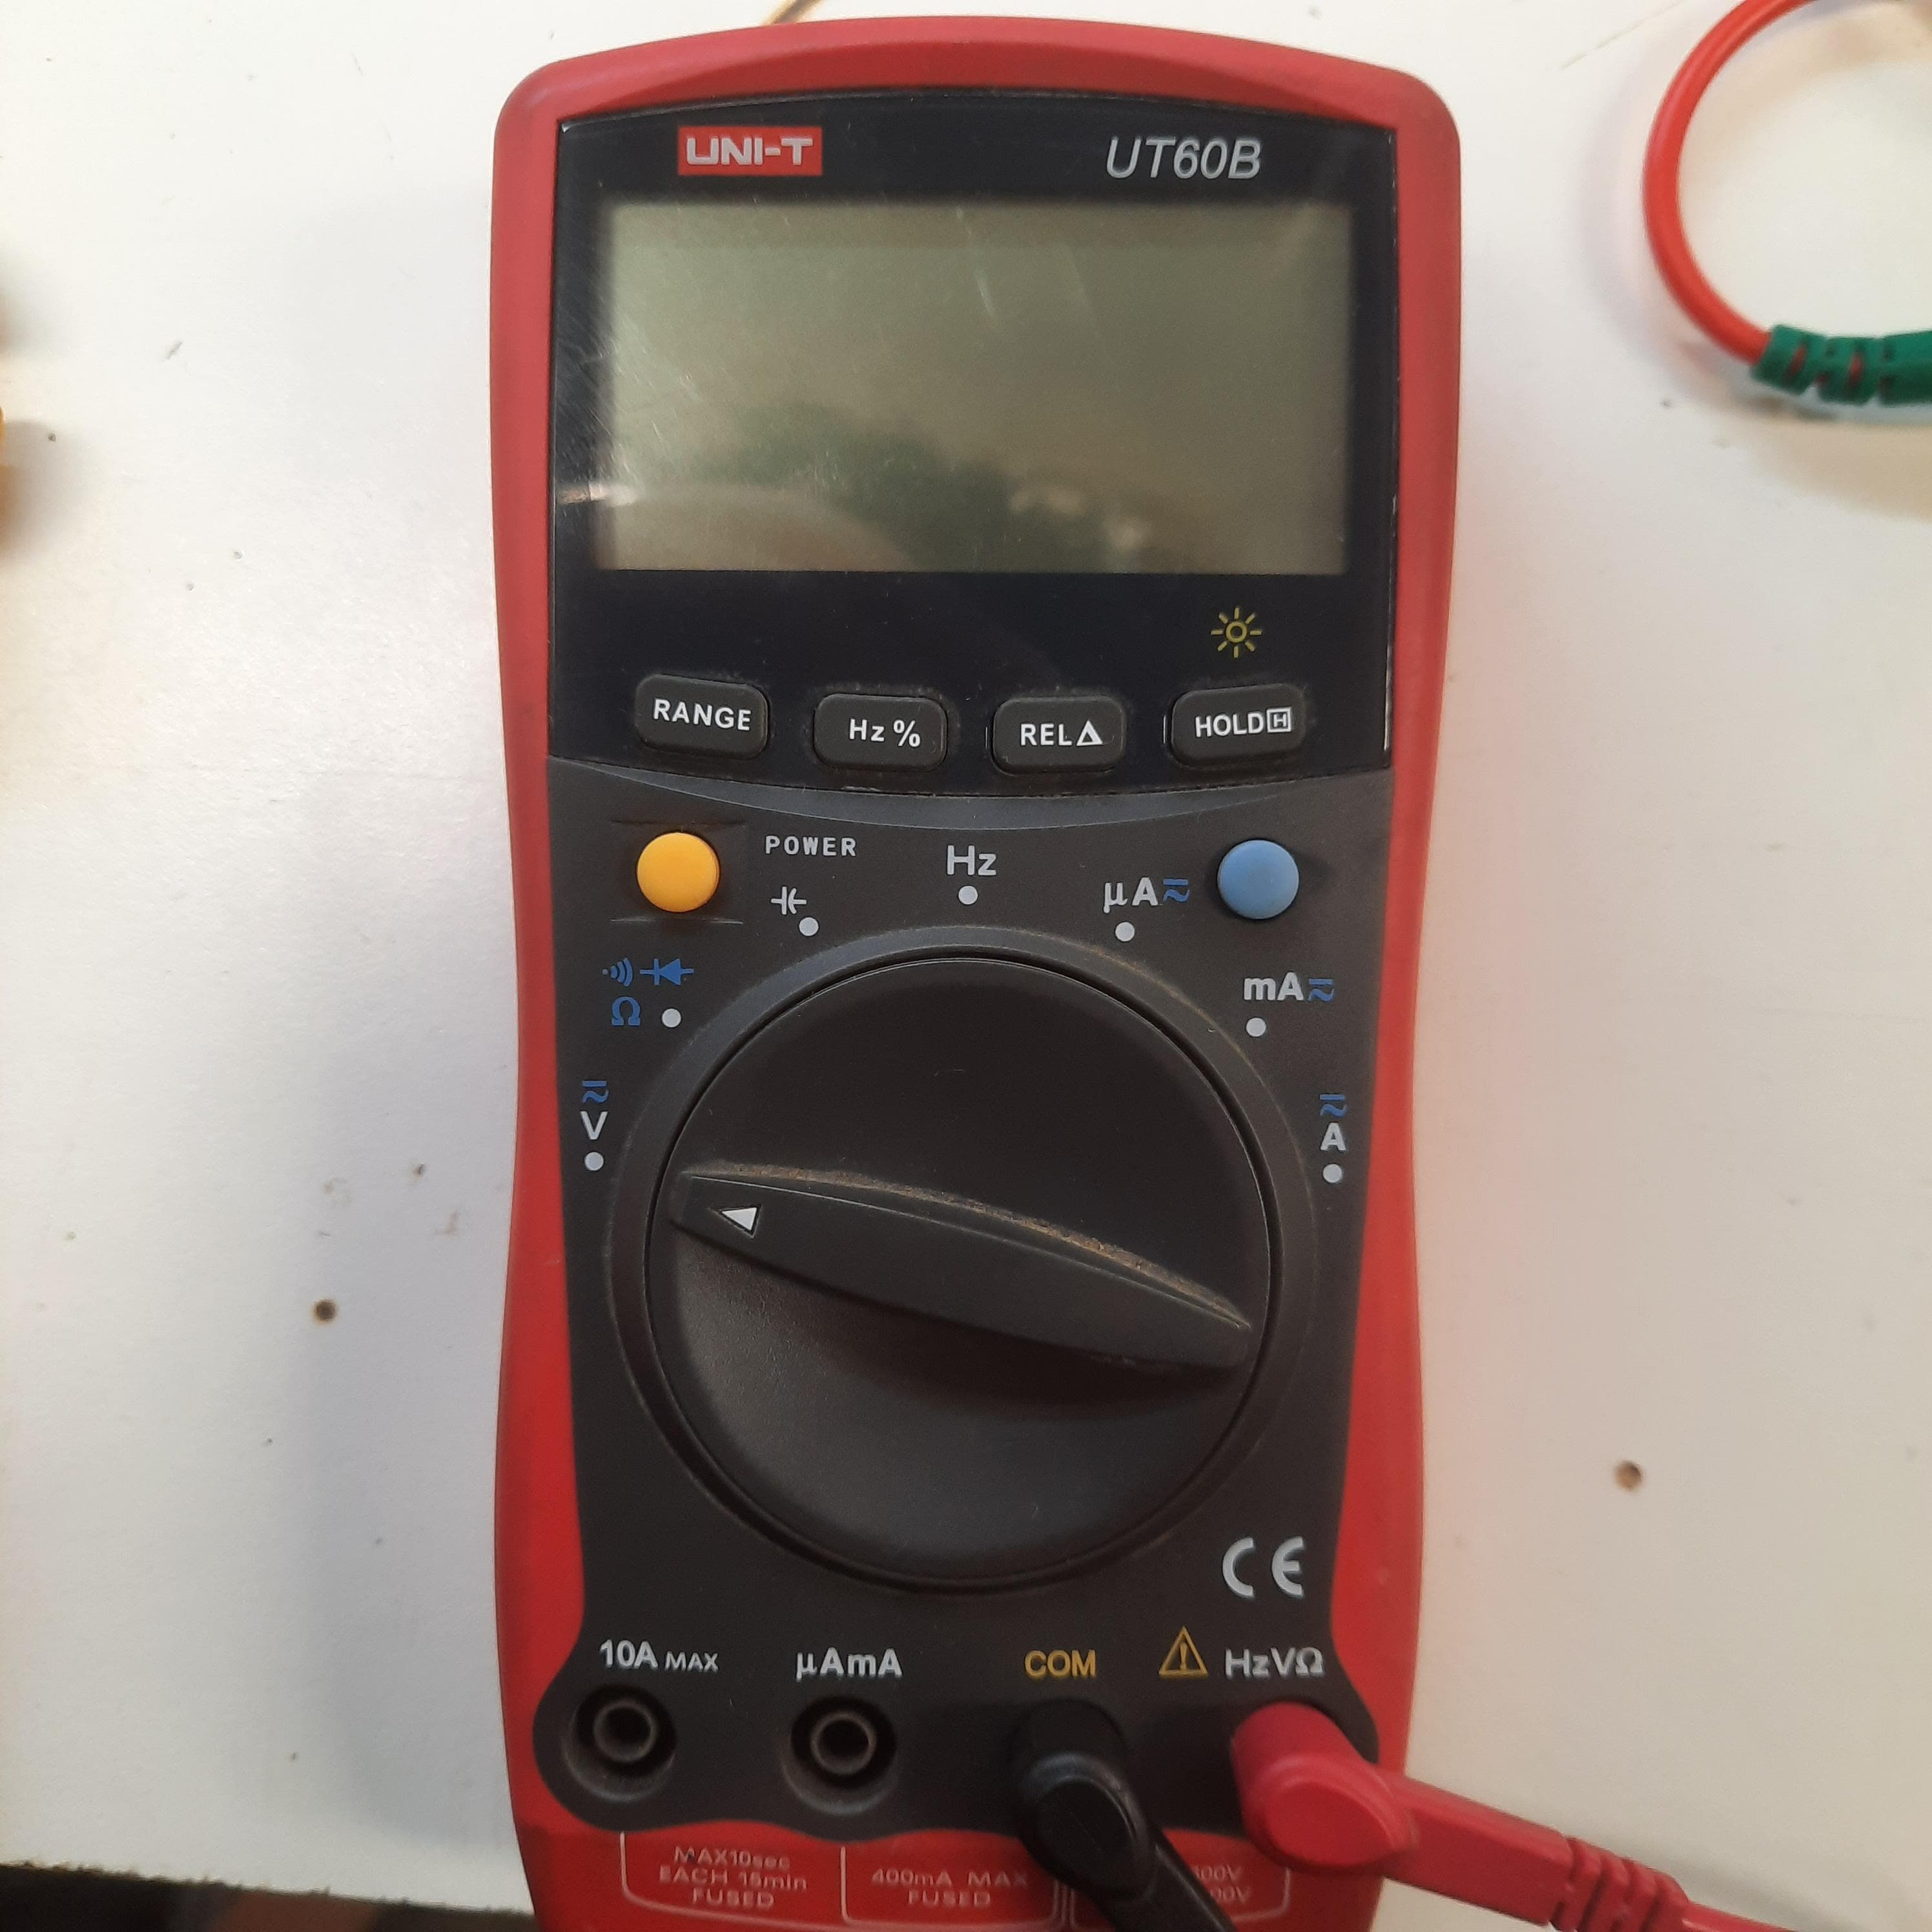
\includegraphics[width=\linewidth]{./imagenes/multimetroRaoMiAmor.jpg}
    \caption{Multimetro 2}
  \end{subfigure}
  \caption{Instrumentos}
  \label{fig:coffee}
\end{figure}

\end{center}

{1) \underline{Multímetro}
\begin{itemize}[nosep]
    \item \textbf{Fabricante:} Pro'sKit
    \item \textbf{Modelo:} MT-1706 CAT 1000V
    \item \textbf{Serie:} MT-17XX
\end{itemize}
\begin{center}
    \begin{tabular}{| p{1cm}  p{1cm}  |}
        \hline
        \multicolumn{2}{|c|}{\textbf{Información de mediciones}} \\
        \hline
        \multicolumn{1}{|m{4cm}}{\centering\textbf{Tensión CC} \\ 60V - Res: 10mV} &
        \multicolumn{1}{|m{3cm}|}{\centering$\pm 0,5\%$ \\+ $3$ dig.} \\
        \hline
        \multicolumn{1}{|m{4cm}}{\centering\textbf{Temperatura $[^oC]$} \\ -20 a 1000$^oC$ - Res: $1^oC$} &
        \multicolumn{1}{|m{3cm}|}{\centering$\pm1,0\% lectura$ \\+ $3$ dig.} \\
        \hline
        \multicolumn{1}{|m{4cm}}{\centering\textbf{hFE{\footnotesize{} [npn, pnp]}} \\ $ I_B \sim 10\mu A$ \\ $V_{CE} \sim 2,8V$} &
        \multicolumn{1}{|m{3cm}|}{\centering $0 \sim 2000$} \\
        \hline
        \multicolumn{1}{|m{4cm}}{\centering\textbf{Corriente continua} \\ $6mA$ - Res: $0,001mA$ \\ $60mA$ - Res: $0,01mA$} &
        \multicolumn{1}{|m{3cm}|}{\centering $\pm$ ($0,8\%$ Lectura + 3dig.)} \\
        \hline

    \end{tabular}
\end{center}

{2) \underline{Multímetro}}
\begin{itemize}[nosep]
    \item \textbf{Fabricante:} UNI-T
    \item \textbf{Modelo:} UT60B
    \item \textbf{Serie:} UT60
\end{itemize}
\begin{center}
    \begin{tabular}{| p{1cm}  p{1cm}  |}
        \hline
        \multicolumn{2}{|c|}{\textbf{Información de mediciones}} \\
        \hline
        \multicolumn{1}{|m{4cm}}{\centering\textbf{Tensión CC} \\ Autorango(400mV-4V)} &
        \multicolumn{1}{|m{3cm}|}{\centering$\pm 0,5\%$ \\+ $1$ dig.} \\
        \hline
        \multicolumn{1}{|m{4cm}}{\centering\textbf{Corriente continua} \\ Autorango(400$\mu A$-4000$\mu A$)} &
        \multicolumn{1}{|m{3cm}|}{\centering $\pm$ ($1\%\sim 3dig$ Lectura + 3dig.)} \\
        \hline
    \end{tabular}
\end{center}


\imagen[Fuente de alimentación UNIT-T]{6cm}{./imagenes/fuenteAlimentacionGod.png}
\begin{itemize}[nosep]
    \item \textbf{Fabricante:} UNIT-T
    \item \textbf{Modelo:} UTP3315TFL-II
    \item \textbf{Serie:} UTP3313TFL-II / UTP3315TFL-II
\end{itemize}
\begin{center}
    \begin{tabular}{| p{1cm}  p{1cm}  |}
        \hline
        \multicolumn{2}{|c|}{\textbf{Información de valores}} \\
        \hline
        \multicolumn{1}{|m{4cm}}{\centering\textbf{Tensión Output} \\ 0 a 30V $V_{CC}$} &
        \multicolumn{1}{|m{3cm}|}{\centering $0,5\%$ + $20mV$} \\
        \hline
        \multicolumn{1}{|m{4cm}}{\centering\textbf{Corriente Output} \\ 0 a 5A} &
        \multicolumn{1}{|m{3cm}|}{\centering$0,5\%$ + $10mA$} \\
        \hline
        \multicolumn{1}{|m{4cm}}{\centering\textbf{Ondulación y ruido}} &
        \multicolumn{1}{|m{3cm}|}{\centering $2mV_{RMS}$} \\
        \hline
    \end{tabular}
\end{center}

\thispagestyle{fancy}

\valentinoQuitaLasColumnas{}
\subsection[Datasheets]{}
\begin{center}
    \begin{tikzpicture}[remember picture, overlay]
        \pgftransformshift{\pgfpoint{0cm}{0cm}}
        \node at (0cm, -10cm) {
\includegraphics[width=10cm]{./imagenes/dibujoDatasheet.jpg}};
        \node at (0cm, -14cm){\Huge\textbf{\textit{DataSheets}}};
    \end{tikzpicture}
\end{center}


\valentinoPoneLasColumnas{}
